%+210 to left and -210 to right if I want to move one subfigure.
\begin{figure}[!h]
%\vspace{-1pt} %takes away some white space before figure
\centering
\begin{subfigure}[b]{0.85\textwidth}
\centering
	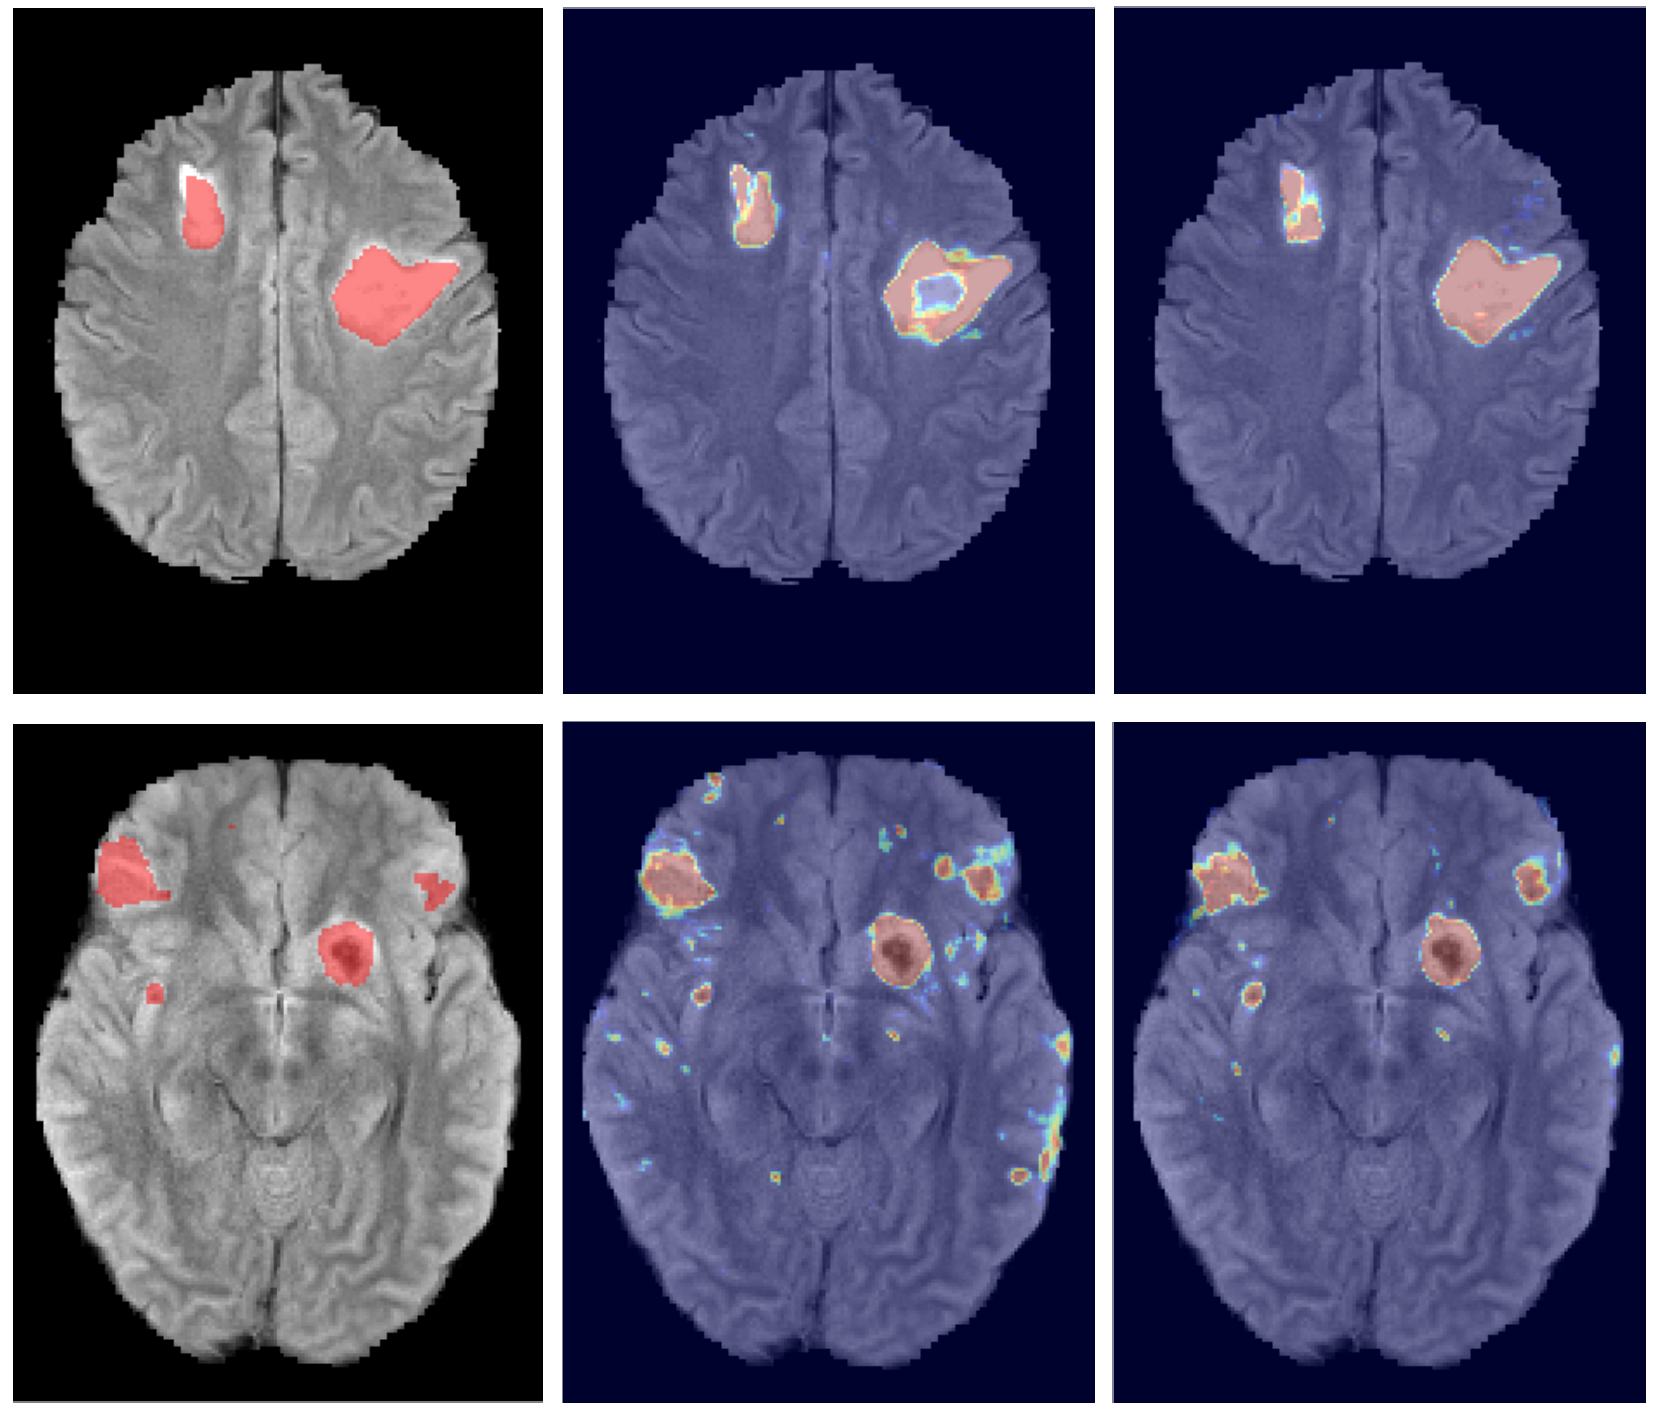
\includegraphics[clip=true, trim=0pt 0pt 0pt 0pt, width=1.0\textwidth]{figures/validationOfArchitecture/multiscale/qualitativeComparisonMultiscale/figureNew/multiscaleQual.png}
\end{subfigure}

\caption{(Rows) Two cases from the severe TBI dataset, showing representative improvements when using the multi-scale CNN approach. (Columns) From left to right: the MRI FLAIR sequence with the manually labeled lesions, predicted soft segmentation map obtained from a single-scale model (Deep\texttt{+}) and the prediction of the multi-scale DeepMedic model. The incorporation of greater context enables DeepMedic to identify when it processes an area within larger lesions (top). Spurious false positives are significantly reduced across the image on the bottom.}
\label{fig:qualitativeMultiscaleVal}
\end{figure}
%\vspace{-1pt} %takes away some white space before figure